\section{Proportional Gain}
In a first approach in controlling this system a proportional gain was installed. The gain will be used in further sections to find the parameters for a PID controller by using the Ziegler-Nichols method.

The simulation was taken with different values for gain. All of the results are plotten in \autoref{fig:prop_gain_non_linearized}
\begin{figure}[H]
    \centering
    \subfigure[$\text{gain }=1$]{\label{fig:prop_gain_non_linearized_g1}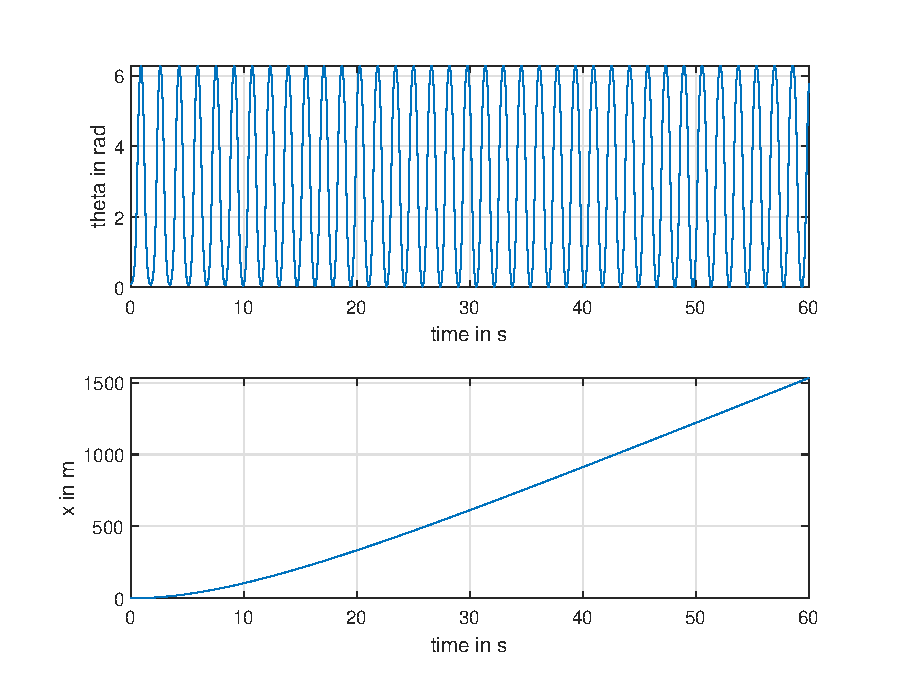
\includegraphics[width=0.49\textwidth]{Lab_report/pics/plots/non_linear_control_g1.eps}}
    \subfigure[$\text{gain }=5$]{\label{fig:prop_gain_non_linearized_g5}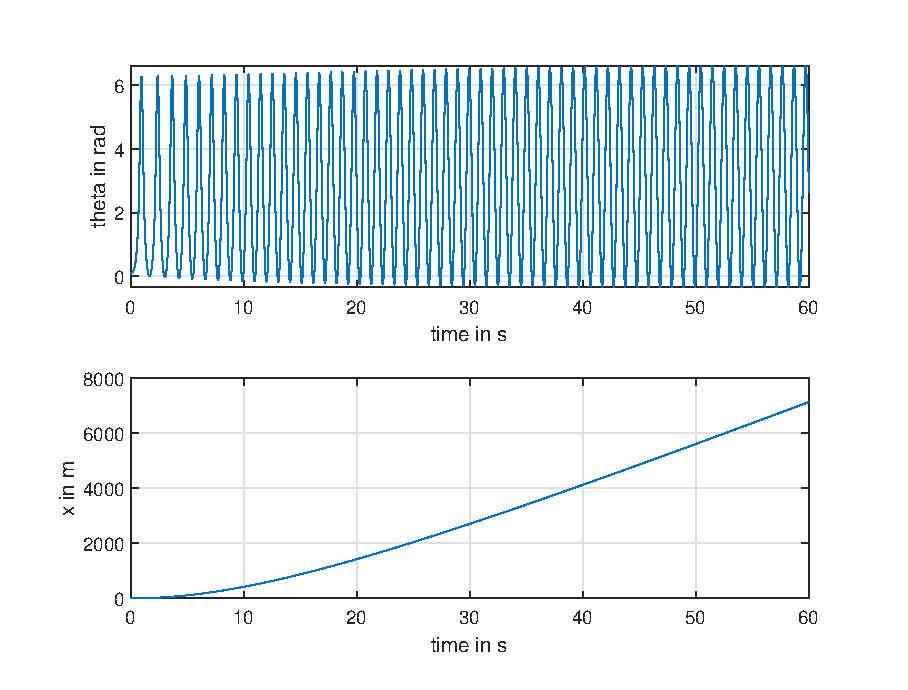
\includegraphics[width=0.49\textwidth]{Lab_report/pics/plots/non_linear_control_g5.eps}}
    \subfigure[$\text{gain }=10$]{\label{fig:prop_gain_non_linearized_g10}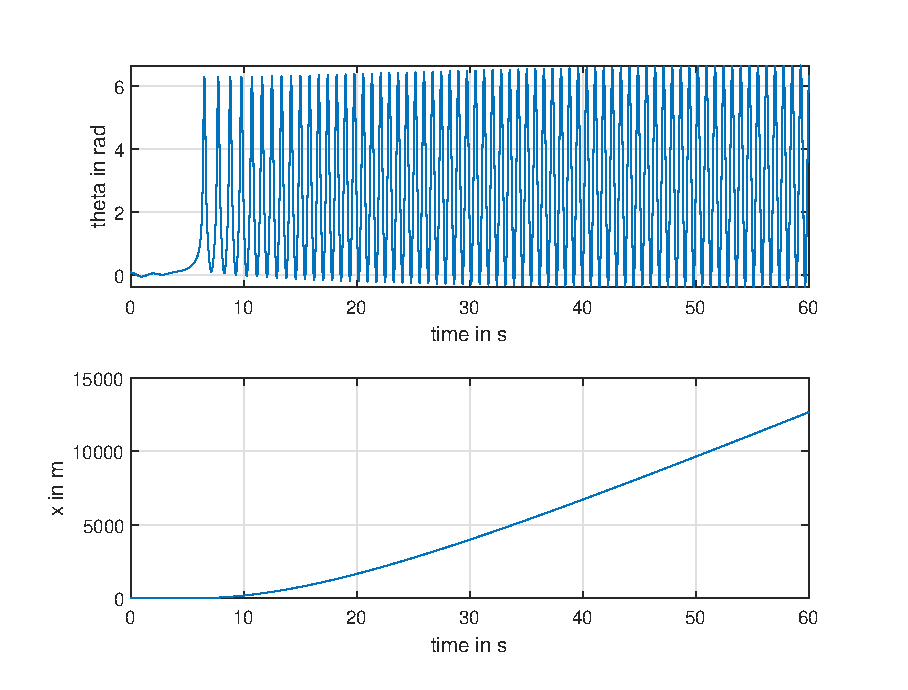
\includegraphics[width=0.49\textwidth]{Lab_report/pics/plots/non_linear_control_g10.eps}}
    \subfigure[$\text{gain }=15$]{\label{fig:prop_gain_non_linearized_g15}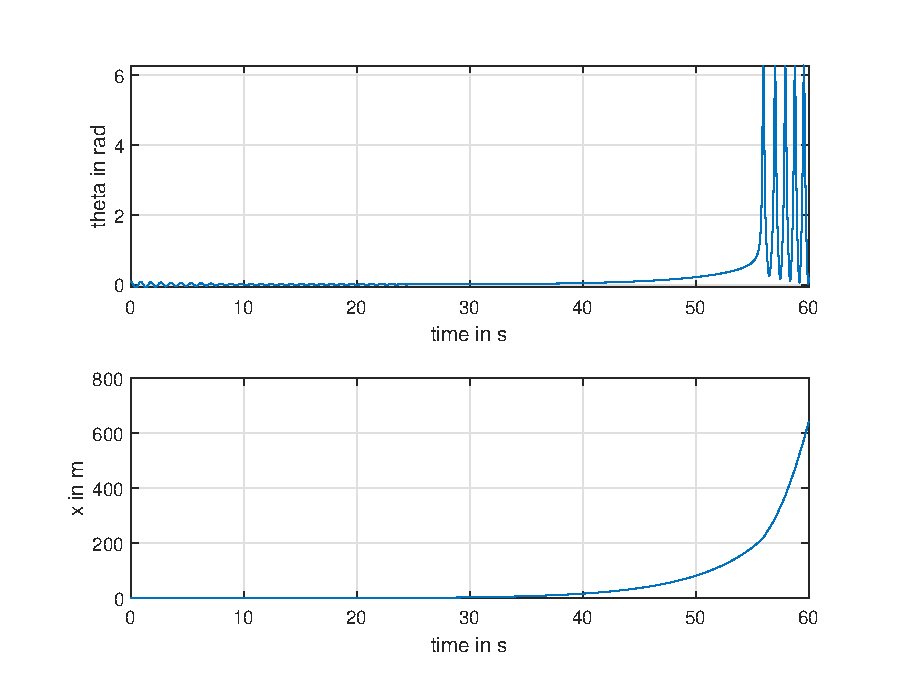
\includegraphics[width=0.49\textwidth]{Lab_report/pics/plots/non_linear_control_g15.eps}}
    \subfigure[$\text{gain }=20$]{\label{fig:prop_gain_non_linearized_g20}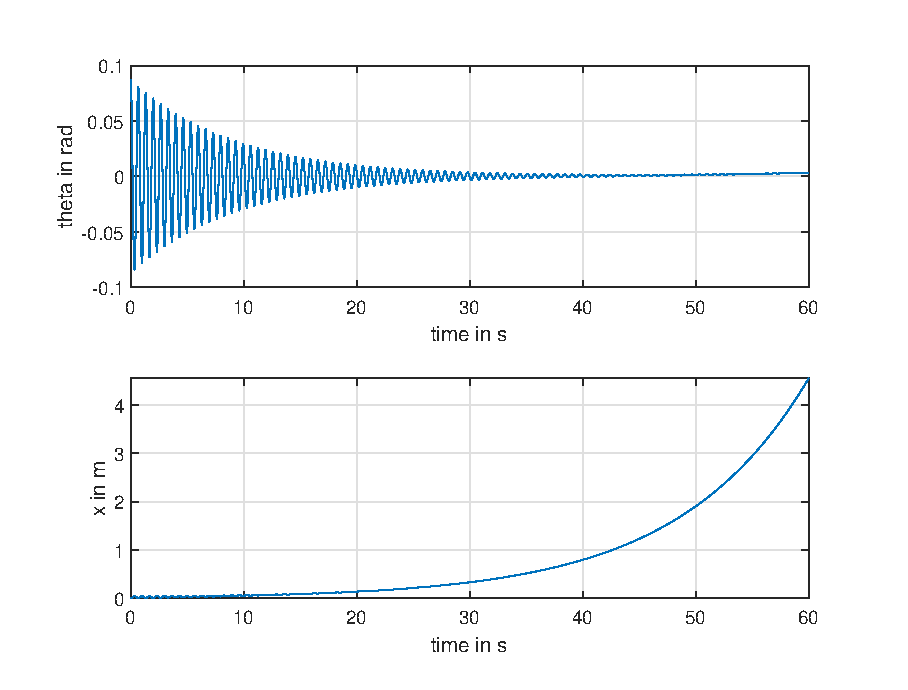
\includegraphics[width=0.49\textwidth]{Lab_report/pics/plots/non_linear_control_g20.eps}}
    \subfigure[$\text{gain }=22.5$]{\label{fig:prop_gain_non_linearized_g22_5}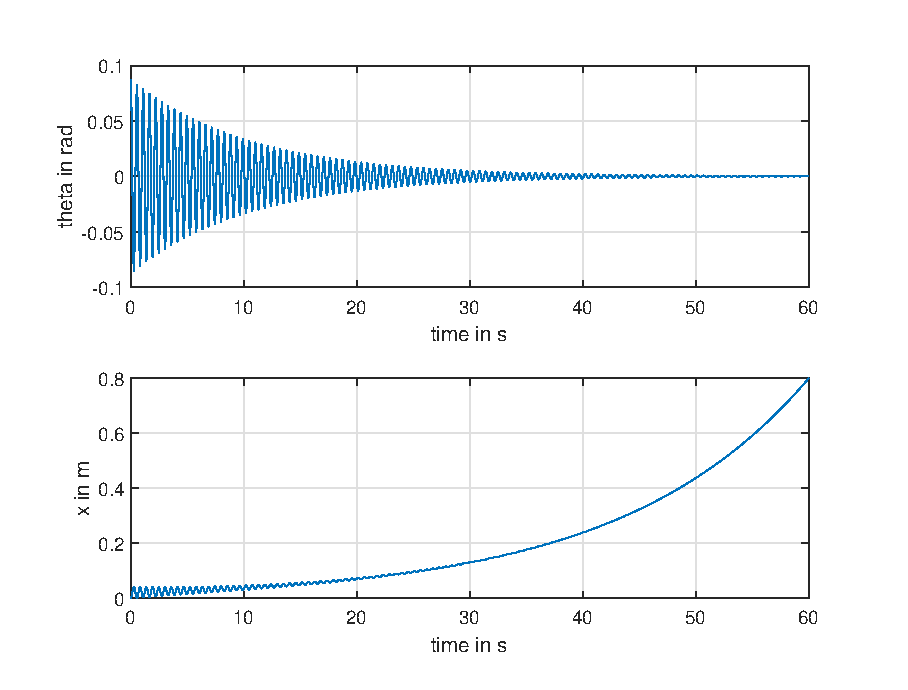
\includegraphics[width=0.49\textwidth]{Lab_report/pics/plots/non_linear_control_g22_5.eps}}
    \caption{simulation results of non linearized Model}
    \label{fig:prop_gain_non_linearized}
\end{figure}

% Please add the following required packages to your document preamble:
% \usepackage[table,xcdraw]{xcolor}
% If you use beamer only pass "xcolor=table" option, i.e. \documentclass[xcolor=table]{beamer}
\begin{table}[H]
\centering
\caption{oscillation periods and stable response, when simulation non-linearized systems with different $k_p$}
\label{tab:sim_res_non_linearized_kp}
\begin{tabular}{|l|l|l|}
\hline
\rowcolor[HTML]{C0C0C0} 
$k_p$ & $T_{osc} \text{in sec}$ & stable response (Y/N) \\ \hline
1     & $1.754$                 & N                     \\ \hline
5     & $1.390$                 & N                     \\ \hline
10    & $1.195$                 & N                     \\ \hline
15    & $1.118$                 & N                     \\ \hline
20    & $0.936$                 & N                     \\ \hline
22.5  & $0.870$                 & N                     \\ \hline
\end{tabular}
\end{table}